%%
%% Meta: Master Document
%% Kompendium GESO
%%

%% Philipp G Freimann Juli 2019 für die BBW
%% Phi BBW-Vorlage für Mathematische Dokumente (LaTeX)
%% 2019 - 07 - 11

%%  In den Dokumenten können die folgenden Attribute überschrieben werden:

%%%%%%%%%%%%%%%%%%%%%%% P A C K A G E S %%%%%%%%%%%%%%%%%%%%%%%%%%%%%
\documentclass[twoside,14pt,a5paper]{extarticle}
\usepackage[paper=a4paper,margin=17mm]{geometry}%

%% Zentralisiert
%%\usepackage{german} %% Macht Probleme mit grafiken
\usepackage{mciteplus}

\usepackage[dvipsnames,table]{xcolor}

\usepackage{pgfplotstable}
\usepackage{tikz}
\usepackage{tkz-euclide} %% Grid

\usepackage{amsthm}
\usepackage{amsfonts} %% Zahlmengen Z, R, ...


%% THEOREMS?
\usepackage{tcolorbox}
\tcbuselibrary{theorems}
\tcbuselibrary{skins}


\usepackage{fancyhdr}
\usepackage{ngerman}
\usepackage[utf8]{inputenc}


%%\usepackage[dvips]{graphicx}

\usepackage{supertabular}
\usepackage{makeidx}  
\usepackage{ifthen} 

\usepackage{multirow}
\usepackage{listings}

%%\usepackage{color,fancyvrb,fancybox}
\usepackage{multicol}
\usepackage{lastpage}
%%\usepackage{listings}
\usepackage{pstricks}

%% bold typewriter font:
\usepackage[T1]{fontenc}
\usepackage{lmodern}

\usepackage{enumitem}
%\usepackage{enumerate}

\usepackage{float}

\usepackage{titlesec}
\usepackage{textcomp}

%% Kuchendiagramme
%%\usepackage{datapie}

%% für Aufgaben Hervorhebung
%%\usepackage[most]{tcolorbox}
%%\usepackage[standard,framed]{ntheorem}
\usepackage{framed}
\usepackage{mdframed}

%%%%%%%%%%%%%%%%%%%%
%%\usepackage[most]{tcolorbox}

\usepackage[tocindentauto]{tocstyle}

%% für accentset wedge:
\usepackage{accents}

%% Würfel
\usepackage{epsdice}

%% Einbinden von GeoGebra Bildchen:
\usetikzlibrary{shapes.geometric}
\usetikzlibrary{arrows}
\newcommand{\degre}{\ensuremath{^\circ}}

%% Hyperlinks
\usepackage{hyperref}

\hypersetup{
    colorlinks=true,
    linkcolor=blue,
    filecolor=magenta,      
    urlcolor=cyan,
    bookmarks=true,
}

%% bugtracker (part of pgfplots) should be loaded AFTER "hyperref"
%% See: https://texblog.net/hyperref/ AND https://tex.stackexchange.com/questions/16268/warning-with-footnotes-namehfootnote-xx-has-been-referenced-but-does-not-exi
\usepackage{pgfplots}
\pgfplotsset{width=10cm,compat=1.9}

%%\usepackage{fourier}  %% eg overarc (Bogenmaß)

%%%%%%%%%%%%%%%%% L A Y O U T  %%%%%%%%%%%%%%%%%%%%%%%%%%%%
%% 2020-12-27 ph. g. freimann @ bbw.ch
%%

\fancyhf{}%%

\pagestyle{fancy}%%

\renewcommand{\sectionmark}[1]{%%
  \markboth{\thesection{} \ #1}{}%%
}%%

\renewcommand{\subsectionmark}[1]{%%
  \markright{\thesubsection \ #1}%%
}%%

%% Achtung: chaptermark nur im BOOK-Style

\renewcommand{\footrulewidth}{0.4pt}

\parskip4pt
\parindent0pt

\topmargin-2.0cm
\textheight24.4cm

\renewcommand{\arraystretch}{1}%%


\newenvironment{bbwFillInTabular}{%%
%% BEGIN PART:
\renewcommand{\arraystretch}{2.1}
\begin{tabular}%%
}%% END PART:
{\end{tabular}
\renewcommand{\arraystretch}{1}%%
}%% END Environment bbwFillInTabular

%%%%%%%%%%%%%%%%%%%%%%%%%%%%%%%%%%%%%%%%%%%%%%%%%%%%%%%%%%
%%%%%%%%%%%%%%%%%% M A K R O S %%%%%%%%%%%%%%%%%%%%%%%%%%%
%%%%%%%%%%%%%%%%%%%%%%%%%%%%%%%%%%%%%%%%%%%%%%%%%%%%%%%%%%

%%%%%%%%%%%%%%%%%%%%%%%% g e n e r e l l e   M a k r o s %%%%%%%%%%%%%%%%%%%%%%%

%% Info vorab bei \newcommand
%% \newcommand{ - Kommandos können in den Parametern auch Leerzeilen
%%     enthalten
%% \newcommand*{ - Kommandos, also mit *, können jedoch in den
%%    Argumenten KEINE \par (sprich Leerzeilen} enthalten

%% 2019-07-26
%% phi@freimann.eu
%% Makros for BBW-Tex Documents
\usepackage{inputs/bbwColors}

%%%%%%%%%%%%%%%%%% I N C L U D E S   &   I N D E X  %%%%%
\graphicspath{{../img/}}
\graphicspath{{./img/}}

\newcommand*\bbwGraphicRaise[3]{\raisebox{#1}{\includegraphics[width=#2]{#3}}}%%
\newcommand*\bbwGraphic[2]{\bbwGraphicRaise{-5mm}{#1}{#2}}%%
\newcommand*\bbwCenterGraphicRaise[3]{\begin{center}\bbwGraphicRaise{#1}{#2}{#3}\end{center}}
\newcommand*\bbwCenterGraphic[2]{\bbwCenterGraphicRaise{-5mm}{#1}{#2}}%%


%% All in one Skript
\newif\ifisALLINONE
\isALLINONEfalse

%% Blended Learning
%% Insb. MatheNinja Links. Diese sind jedoch in einem anderen Kurs!
\newif\ifisBLENDED
\isBLENDEDfalse


%%%%%%%%% TRAINER Version vs. Schülerversion %%%%%%%%%%%%%
%% Bem. Kein *-Kommando, da die TRAINER-Blöcke auch leerzeilne (\par)
%% enthaltne können
\newcommand\TRAINER[1]{%%
{%%
\ifisTRAINER{\color{BlueGreen}{#1}}%%
\fi%%
}}%%  

\newcommand\TALS[1]{%
{%%
\ifisTALS{#1}%%
\fi%%
}}%

\newcommand\GESO[1]{%
{%%
\ifisGESO{#1}%%
\fi%%
}}%    

\newcommand\BLENDED[1]{%
{%%
\ifisBLENDED{#1}%%
\fi%%
}}%    

\newcommand{\noTRAINER}[1]{{\ifisTRAINER{}\else{#1}\fi}{}}%%



%%\makeatletter
%% Je nach Umgebung "environment" wird das mmPapier breiter oder
%% schmaler
%% bei itemize sollen 16.4 und bei definiton-Boxen 16.8 mm genommen
%% werden.


\usepackage{inputs/mmPapierbreiteSty}


%% Trainer "no" Dotfill
%% If no Trainer: Dotfill
\newcommand*{\TNDF}[1]{\TRAINER{#1}\noTRAINER{\dotfill{}}}%%

\newcommand*{\leserluft}{\vspace{2mm}}

%% Notiz felder 
%% Anwendung:
%% \noteField{10}  
%%  --> Notizfeld mit 10 Leerzeilen
\newcounter{DFCounter}


%%Häuschenpapier
\newcommand{\mmPapierZwei}[2]{\begin{tikzpicture}
%%  \draw[step=4mm,bbwMMFarbe,ultra thin]
%%  \draw[step=4mm,bbwMMFarbe,thick]
  \draw[step=4mm,bbwMMFarbe,line width=0.02mm]
  (0, 0) grid ({#2}, {#1});
\end{tikzpicture}}%%


%% millimeterPapier füllen bis Ende Seite
\newcommand{\mmPapierBisEndeSeite}{

\begin{tikzpicture}

\newdimen\spaceleftOnPage
\spaceleftOnPage=\dimexpr\textheight-\pagetotal-14pt\relax

\pgfmathsetmacro{\gridWidth}{\textwidth        - mod(\textwidth,      4mm)      }
\pgfmathsetmacro{\gridHeight}{\spaceleftOnPage - mod(\spaceleftOnPage,4mm) - 4mm}

\draw [step=4mm,bbwMMFarbe,line width=0.02mm] (0,0) grid (\gridWidth pt,\gridHeight pt);
\end{tikzpicture}%%
\newpage%%
}%% END Makro mmPapieBisEndeSeite


%% Standardbreite für Arbeitsblätter und das Theorieheft
%% Wird in bbwPruefung.sty überschrieben, da dort schmaler
\def\defaultTextBreite{17.6}
\def\unitCMWhatElse{cm}%% wird als Breitenangabe für den nächsten command verwendet

%% Verwendung: \bbwCenterGraphic{\defaultTextBreite}{«img url»}
\def\defaultTextBreiteCM{\defaultTextBreite\unitCMWhatElse}
\newcommand{\mmPapier}[1]{\mmPapierZwei{#1}{\defaultTextBreite}}


%% Notizen Berechungen auf Prüfungsblättern
\newcommand{\platzFuerBerechnungen}[1]{\noTRAINER{

Notizen / Berechnungen:

\mmPapier{#1}}}%% end platzFuerBerechnungen

\newcommand{\platzFuerBerechnungenBisEndeSeite}[1]{\noTRAINER{

Notizen / Berechnungen:

\mmPapierBisEndeSeite}}%% end platzFuerBerechnungen



\newcommand{\platzFuerBerechnungenOhneText}[1]{\noTRAINER{

\mmPapier{#1}}}

%% Die Abkürzung z.\,B. von «Zum Beispiel» hat einen verkleinerten Abstand.
\newcommand*\zB{%
z.\,B.
}

%%
%% Auf der Titelseite steht entweder GESO oder TALS.
%% Dies wird gleich mit der Fußnote angegeben.
%% Dieses Kommando sollte im Kommando «\untertitel» eingesetzt werden.
%%
\newcommand*\ausrichtungAufTitelseite{%
\ifisTALS{TALS\noTRAINER{\footnote{TALS «Technik, Architektur und Life Sciences
(Laboranten)»: Ausrichtung technisches Profil}}}%%
\fi%%
\ifisGESO{GESO\noTRAINER{\footnote{GESO: Ausrichtung \textbf{Ge}sundheit und \textbf{So}ziales}}}%%
\fi}%%

%%%%%%%%%%%%%%%%%%%%%% B B W - M a t h e   F a r b c o d e s  %%%%%%%%%%%%%%%%%%%%%%%%%%%%%%555

\newcommand{\rezeptFarbe}{rezeptFarbe}
\newcommand{\definitionFarbe}{definitionFarbe}
\newcommand{\gesetzFarbe}{gesetzFarbe}
\newcommand{\beispielFarbe}{beispielFarbe}
\newcommand{\bemerkungFarbe}{bemerkungFarbe}

%% Falls gewünscht übersteuren
%  \definecolor{xyz}{HTML}{eeff66}
%  \renewcommand{\beispielFarbe}{xyz}
%

%% Theorem-Styles
\newcommand\theoremlayoutdefinition[4]{\newtcbtheorem[number within=section]{#1}{#2}%
   {theorem style=plain,enhanced,colframe=#3!20!white,colback=#3!20!white,
     coltitle=#3!60!black,fonttitle=\upshape\bfseries,
     %%fontupper=\itshape,
    %%drop fuzzy shadow=blue!50!black!50!white,
    terminator sign={:},
    borderline north={0.5mm}{0pt}{#3}, borderline south={0.5mm}{0pt}{#3}
}{#4}}



%% Farben für rezept, definition und gesetz von Marthale übernommen.
%% Verwendung mit * unterbindet die Nummerierung \begin{gesetz*}{Blah}{xy} ...\end {gesetz*}
\theoremlayoutdefinition{rezept}{Rezept}{\rezeptFarbe}{R}
\theoremlayoutdefinition{definition}{Definition}{\definitionFarbe}{D}
\theoremlayoutdefinition{gesetz}{Gesetz}{\gesetzFarbe}{G}%% was green
\theoremlayoutdefinition{beispiel}{Beispiel}{\beispielFarbe}{B}
\theoremlayoutdefinition{bemerkung}{Bemerkung}{\bemerkungFarbe}{M}

%%
%% Force a blank page, when \newpage does not work
%%
\def\blankpage{%
	\clearpage%
	\null%
	\clearpage}%%

\newcommand{\Lueckentext}[1]{\,\,\noTRAINER{\dotfill}\TRAINER{#1}}


\newcommand{\LoesungsRaumCM}[2]{\,\,\noTRAINER{\underline{\hspace{#1}}}\TRAINER{#2}}

\newcommand{\LoesungsRaum}[1]{\LoesungsRaumCM{30mm}{#1}}
\newcommand{\LoesungsRaumKurz}[1]{\LoesungsRaumCM{15mm}{#1}}
\newcommand{\LoesungsRaumLang}[1]{\LoesungsRaumCM{45mm}{#1}}


%% TI nSpire
\def\tinspire{\texttt{TI-nSpire}}

%% TI 30 Pro Mathprint Button Images
\def\tiprobuttonbreite{10mm}
\def\nspirebuttonbreite{8.6mm}

%%\def\sec{\raisebox{-2mm}{\includegraphics[width=\buttonbreite{}]{img/tiprobuttonimages/2nd.png}}}
\newcommand{\tiprobutton}[1]{\raisebox{-2mm}{\mbox{\,\includegraphics[width=\tiprobuttonbreite{}]{img/tiprobuttonimages/#1.png}\,}}}

\newcommand{\nspirebutton}[1]{\raisebox{-2mm}{\mbox{\,\includegraphics[width=\nspirebuttonbreite{}]{img/nspirebuttonimages/#1.png}\,}}}

%% Counter  für Aufgaben
%% Bei jedem Part wird die Aufgabennummer zurückgesetz auf 1
\newcommand{\bbwPartID}{AA1}
\newcommand{\bbwAufgabenBlockID}{}
\newcounter{bbwAufgabenNummerCounter}[part]
\setcounter{bbwAufgabenNummerCounter}{1}
\newcommand{\bbwAufgabenNummer}{\arabic{bbwAufgabenNummerCounter}}
\newcommand{\nextBbwAufgabenNummer}{\stepcounter{bbwAufgabenNummerCounter}}
\newcommand{\aufgSubLabel}{{\color{blue}\bbwAufgabenNummer. \alph*)}}

%% Benutze außerhalb der bbwAufgabenblöcke folgendes Kommando, um an die
%% nächste Aufgabennummer zu kommen. Dies z. B. wenn ein längerer Text vor der Aufgabe steht,
%% der auch schon diese Bezeichnung erhalten sollte
\newcommand{\bbwActAufgabenNr}{{\color{blue}\bbwAufgabenNummer. {\small[\bbwAufgabenBlockID]}}}


\newenvironment{bbwAufgabenBlock}{%% Begin environment Part:

\bbwActAufgabenNr{}
%%{\color{blue}\bbwAufgabenNummer. {\small[\bbwAufgabenBlockID]}}
\begin{enumerate}[label=\aufgSubLabel]
}%% Ende der Präambel
{%% END Part:
\end{enumerate}
\nextBbwAufgabenNummer
}%% END environment bbwAufgabenBlock

%%%%%%%%%%%%%%%%%%%%%%%%%%%%

%% Weblinks und Mathe Ninja Links

\newcommand{\weblink}[2]{\href{#2}{#1}}

\newcommand{\olatBBWLogo}{
\includegraphics[width=15mm]{logos/traube.pdf}}%%
\newcommand{\externerLinkEPS}{
\includegraphics[width=15mm]{logos/extLink.pdf}}%%
\newcommand{\youtubeLogo}{\includegraphics[width=15mm]{logos/youtube.png}}%%


%%
%% #1: Text
%% #2: URL
%% #3: Aufgabennummern
%% #4: optional weitere Logos oder leer lassen {}
\newcommand{\externalLink}[4]{%%
\begin{tabular}{|lp{111mm}|}\hline%%
\multicolumn{2}{|p{172mm}|}{\cellcolor{aufgabenFarbe}#3}\\
\weblink{\raisebox{-5mm}{\externerLinkEPS{}}}{#2} {#4}  & \weblink{#1}{#2}\\\hline
\multicolumn{2}{|p{172mm}|}{\weblink{#2}{#2}}\\\hline
\end{tabular}%%
\vspace{1mm}
}%% END Command externalLink

%% #1: URL
%% #2: Text
\newcommand{\youtubeLink}[2]{%%
\externalLink{#2}{#1}{Youtube}{\raisebox{-5mm}{\youtubeLogo{}}}
}%%

%%
%% #1: Typ-Logo (eg. LOGO auf MatheNinja)
%% #2: Typ-Name (eg «Mathe Ninja»
%% #3: URL
%% #4: Aufgaben Name
\newcommand{\olatLink}[4]{%%
\begin{tabular}{|lp{111mm}|}\hline%%
\multicolumn{2}{|p{172mm}|}{\cellcolor{aufgabenFarbe}#4}\\
\weblink{\raisebox{-5mm}{\externerLinkEPS{}}}{#3} \weblink{\raisebox{-5mm}{\olatBBWLogo}}{#3} \weblink{#1}{#3}& \weblink{#2}{#3}\\\hline
\end{tabular}%%
\vspace{1mm}
}%% END Command olatLink


%\newcommand{\olatLOGOLink}[3]{%%
%\begin{tabular}{|lp{111mm}|}\hline%%
%\weblink{\raisebox{-5mm}{\olatBBWLogo{}}}{#2} & \weblink{#1}{#2}\\
%\multicolumn{2}{|p{172mm}|}{\cellcolor{aufgabenFarbe}#3}\\\hline
%\end{tabular}%%
%}%% END Command olatLOGOLink

%% Use:
%% \olatLinkArbeitsblatt{Kapitel/Arbeitsblattname «[ID]»}{«URL»}{Aufgabennummern}
\newcommand{\olatLinkArbeitsblatt}[3]{\olatLink{\raisebox{-6mm}{
\includegraphics[width=12mm]{logos/seite.pdf}}}{Arbeitsblatt: #1}{#2}{#3}}%%

%% #1: Text
%% #2: URL
\newcommand{\olatLinkPruefung}[2]{\olatLink{\raisebox{-6mm}{
\includegraphics[width=15mm]{logos/test.pdf}}}{Online Test}{#2}{#1}}%%


%%
%% use:
%% \matheNinjaLink{Beschreibung}{URL}
\newcommand{\matheNinjaLink}[2]{\olatLink{\raisebox{-6mm}{\includegraphics[width=17mm]{img/matheninja/matheninja.jpg}}}{Mathe Ninja!}{#2}{#1}}%%


%% Use
%% \olatLinkGESOKompendium{Kapitel}{Seite/Seiteff}{Aufgabe(n)}
\newcommand{\olatLinkGESOKompendium}[3]{%%
\GESO{%%
\olatLink{{\Huge K}}{Kompendium}{https://olat.bbw.ch/auth/RepositoryEntry/572162163/CourseNode/106029172671728}{Kapitel #1; Seite #2; Aufg. #3}%%
}%% END GESO
}%%


%% Use \olatLinkTALSStrukturaufgabenSPF{Kapitel}{Seite/Seiteff}{Aufgabe(n)}
\newcommand{\olatLinkTALSStrukturaufgabenSPF}[3]{%%
\TALS{%%
\olatLink{{\Huge S}}{Strukturaufgaben}{https://olat.bbw.ch/auth/RepositoryEntry/572162090/CourseNode/102901174299246}{Kapitel #1; Seite #2; Aufgaben #3}%%
}%% END GESO
}%%

%%\newcommand{\olatLinkTALtfSStrukturaufgabenGLF}[1]{\olatLOGOLink{Strukturaufgaben Grundlagenfach}{https://olat.bbw.ch/auth/RepositoryEntry/572162090/CourseNode/102901174291476}{#1}}


%%\newcommand{\matheNinjaLink}[2]{%%
%%\begin{tabular}{cc}%%
%% \raisebox{-1cm}{\includegraphics[height=2cm]{img/matheninja/turtle.png}}& \href{#2}{MatheNinja: #1}\\%%
%% \end{tabular}%%
%%}%% End Command  \matheNinjaLink



%% AadB = Aufgaben aus dem Buch
%% 1. Parameter: Seitenzahl
%% 2. Parameter: Aufgabennummern.
%% bsp  \TALSAadB{38-39}{101a-101c, 102 und 103}

%%\newcommand*{\maturaAufgaben}[1]{\begin{mdframed}[backgroundcolor=maturaAufgabenFarbe!10]{#1}\end{mdframed}}

\newcommand*{\aadBTxt}{Aufgaben aus dem Buch}


%%
% Generell Aufgaben aus einem Lehrbuch
% #1: cite auf das Lehrbuch (z. B. frommenwiler17alg)
% #2: Seitennummer oder Seitennumerff
% #3: aufgabennummer(n)
\newcommand*{\AadB}[3]{%%
\aufgabenFarbe{\noindent{\aadBTxt \cite{#1}: Seite {#2} Nr. {#3}}}%%
}%%

%%\newcommand*{\AdbBAlgebra}[2]{\AadB{marthaler21alg}{#1}{#2}}%%

\newcommand*{\TALSAadBFWA}[2]{\ifisTALS{\AadB{frommenwiler17alg}{#1}{#2}}\fi}%%
\newcommand*{\TALSAadBMTA}[2]{\ifisTALS{\AadB{marthaler21alg}{#1}{#2}}\fi}%%
\newcommand*{\TALSAadBFWG}[2]{\ifisTALS{\AadB{frommenwiler18geom}{#1}{#2}}\fi}%%
\newcommand*{\TALSAadBMTG}[2]{\ifisTALS{\AadB{marthaler20geom}{#1}{#2}}\fi}%%

%% GESO hat (noch) keine Geometrie
\newcommand*{\GESOAadBMTA}[2]{\ifisGESO{\AadB{marthaler21alg}{#1}{#2}}\fi}%%

\newcommand*{\AadBMTA}[2]{\AadB{marthaler21alg}{#1}{#2}}
\newcommand*{\AadBMTG}[2]{\AadB{marthaler20geom}{#1}{#2}}

%%
% Generell Theorie aus einem Lehrbuch
% #1: cite auf das Lehrbuch (z. B. frommenwiler17alg)
% #2: Seitennummer oder Seitennumerff
% #3: KapitelNummer
\newcommand*{\TadB}[3]{%%
\aufgabenFarbe{\noindent{Theorie \cite{#1}: Seite {#2} Nr. {#3}}}%%
}%%

\newcommand*{\TALSTadBFWA}[2]{\ifisTALS{\TadB{frommenwiler17alg}{#1}{#2}}\fi}%%
\newcommand*{\TALSTadBMTA}[2]{\ifisTALS{\TadB{marthaler21alg}{#1}{#2}}\fi}%%
\newcommand*{\TALSTadBFWG}[2]{\ifisTALS{\TadB{frommenwiler18geom}{#1}{#2}}\fi}%%
\newcommand*{\TALSTadBMTG}[2]{\ifisTALS{\TadB{marthaler20geom}{#1}{#2}}\fi}%%

%% GESO hat (noch) keine Geometrie
\newcommand*{\GESOTadBMTA}[2]{\ifisGESO{\TadB{marthaler21alg}{#1}{#2}}\fi}%%
\newcommand*{\TadBMTA}[2]{\TadB{marthaler21alg}{#1}{#2}}
\newcommand*{\TadBMTG}[2]{\TadB{marthaler20geom}{#1}{#2}}


%% Referenzen auf Labels
%% AllInOne ist wichtig, denn einige Referenzen funkitionieren nicht
%% in den Themen-Skripts, sondern lediglich in den gesamten Jahres-Skripts.
\newcommand*\totalref[1]{\ifisALLINONE{ (s.\kern 0.22em{}Kap. \ref{#1}
    auf Seite \pageref{#1}) }\else{}\fi{}}%%
\newcommand*\totalrefanhang[1]{ (s.\kern 0.22em{}Kap. \ref{#1}
    auf Seite \pageref{#1}) }%%

%% Short version
\newcommand*\totalrefs[1]{\ifisALLINONE{ Kap. \ref{#1} auf Seite
\pageref{#1} }\else{}\fi{}}%%
%%\newcommand*\aufgabenref[1]{(s\kern 0.22em{}Aufg. \ref{#1} auf Seite \pageref{#1})}

%%%%%%%%%%%%%%%%%%%%%%%%%%%%%%%%%%% BBW Makros %%%%%%%%%%%%%%%%%%%%%%%%%%%%%


%% Philipp G Freimann Juli 2019 für die BBW
%% Phi BBW-Vorlage für Mathematische Dokumente (LaTeX)
%% 2019 - 07 - 11
%%%%%%%%%%%%%%%%%%%%%%%%%%% M a t h e   M a k r o s %%%%%%%%%%%%%%%%%%%%%%%%%%%%%5

\usetikzlibrary{arrows.meta}

%% Kleine Symbole über anderen. Z. B. "?" über einem
%% Gleichheitszeichen:
%% Use \ueberMini{=}{?} um ein kleines Fragezeichen über ein
%% Gleichheitsszeichen zu schreiben.
\newcommand{\ueberMini}[2]{ \mathrel{\stackrel{\makebox[0pt]{\mbox{\normalfont\tiny #2}}}{#1}} }

%% Gleichungssystem mit zwei Zeilen und vier Einträgen (je zwei links
%% bzw. rechts).
\def\gleichungZZ#1#2#3#4{%%
  $$\left|
  \begin{array}{rcl}
    {#1} &=& {#2}\\
    {#3} &=& {#4}
    \end{array}\right|$$}%%

\def\gleichungDD#1#2#3#4#5#6{%%
  $$\left|
  \begin{array}{rcl}
    {#1} &=& {#2}\\
    {#3} &=& {#4}\\
    {#5} &=& {#6}\\
    \end{array}\right|$$}%%

%% Entspricht-Symbol
%%\usepackage{accents}
\newcommand{\hatset}[1]{\accentset{\wedge}{#1}}
\newcommand{\entspricht}{\,\,\hatset{=}\,\,}
\newcommand*\mittelwert[1]{\bar{#1}}
\newcommand*\mediantilde[1]{\widetilde{#1}}

%%
%% Graphiken mit tikz: BBW-Mathe-akros
%%
\tikzset{bbwgrid/.style={help lines,color=cyan!18, step=0.5cm}}

\newcommand{\bbwGridPart}[4]{
 % grid:
 \draw[bbwgrid] (#1,#3) grid (#2,#4);

 % axes
 \draw[thick] (#1,0) -- (#2,0);
 \draw[thick] (0,#3) -- (0,#4);
 \foreach \x in {#1, ..., -1}  \draw (\x cm, 2pt) -- (\x cm, -2pt)  node[anchor=north]{$\x$};
 \foreach \x in {1, ..., #2}   \draw (\x cm, 2pt) -- (\x cm, -2pt)  node[anchor=north]{$\x$};
 \foreach \y in {#3, ..., -1}  \draw (-2pt, \y cm) -- (2pt, \y cm)  node[anchor=east]{$\y\,\,$};
 \foreach \y in {1, ..., #4}   \draw (-2pt, \y cm) -- (2pt, \y cm)  node[anchor=east]{$\y\,\,$};
 \draw[->,thick] (#2,0) -- ({#2+0.5},0) node[anchor=west]{$x$};
 \draw[->,thick] (0,#4) -- (0,{#4+0.5}) node[anchor=south]{$y$};
}


%% A function within a Grid (without painting the grid)
%% #1: funciton eg 2*\x  (x has to be backquoted)
%% #2: Domain eg. -1:2.5
%% #3: colour eg red
\newcommand{\bbwFuncC}[3]{\draw[domain=#2,smooth,samples=200,variable=\x,#3] plot ({\x},{#1});
}
%% A function within a Grid (without painting the grid)
\newcommand{\bbwFunc}[2]{\bbwFuncC{#1}{#2}{blue}}

%% Declare a function-plot
%% xmin,xmax,ymin,ymax,fct,domain(x-min, x-max)
%% example: \bbwFunction{-4}{3}{-2}{5}{-\x*\x- \x + 4.5}{-3:2}
\newcommand{\bbwFunction}[6]{\begin{tikzpicture}
\bbwGridPart{#1}{#2}{#3}{#4}
 \bbwFunc{#5}{#6}
%% \draw[domain=#6,smooth,samples=200,variable=\x,blue] plot ({\x},{#5});
\end{tikzpicture}}
%% a whole graph having a coordinate-system #1-#4 and any tizpicture content #5:
\newcommand{\bbwGraph}[5]{\begin{tikzpicture}\bbwGridPart{#1}{#2}{#3}{#4}#5\end{tikzpicture}}

%% Dots and lines:
%% Dot example: \bbwDot{-1,2}{red}{east}{A}
\newcommand{\bbwDot}[4]{\filldraw[color=#2!60, fill=#2!5, thick](#1) circle(0.05) node[anchor=#3]{$#4$};}

%% Line example: \bbwLine{-1,0}{2,3}{red}
\newcommand{\bbwLine}[3]{\draw[thick,color=#3] (#1)--(#2);}

\newcommand{\bbwArrow}[3]{\draw[thick,color=#3,->] (#1)--(#2);}


%% Draw a single letter or small text
% #1: Position eg  4,4
% #2: letter eg f or blah
% #3: colour
\newcommand{\bbwLetter}[3]{\draw[color=#3](#1) node{$#2$};}

%%% ABC-Formel
%% usage \abcd{<a>}{<b>}{<c>}
%% example usage: \abcd{b}{5}{\sqrt{4}}
\newcommand{\abcd}[3]{$\frac{-(#2)\pm\sqrt{(#2)^2 - 4\cdot{}(#1)\cdot{}(#3)}}{2\cdot{}(#1)}$}



%% Trigonometrische Koordinatensysteme
%% Alle heißen "trigsysS" wobei da S einer der folgenden Sub-Systeme
%% bezeichnet:
%%  A  phi von  0 ... 360
%%     y   von -3 ...   3
%%
%%  B  phi von  0 ... 360
%%     y   von -1 ...   1
%%
%%  C  phi von  -270 ... 450
%%     y   von    -2 ...   2
%%
%%  D  phi von  -270 ... 450
%%     y   von    -1 ...   1
%%

\newcommand{\trigsysA}{
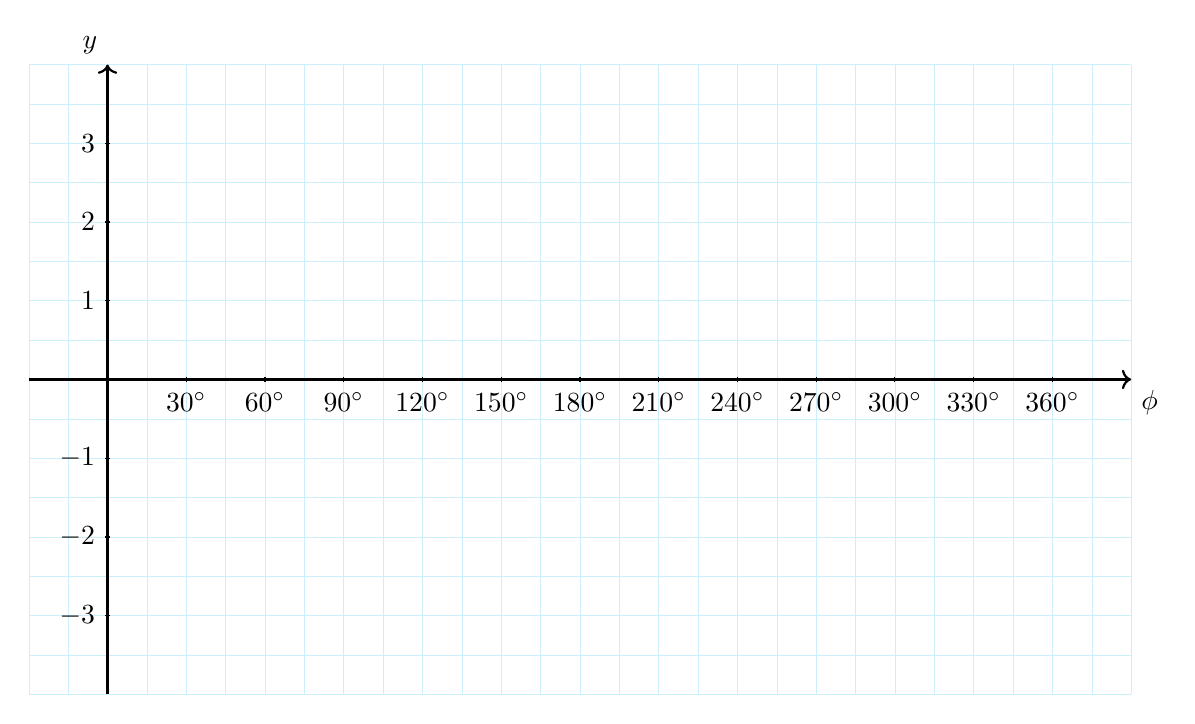
\begin{tikzpicture}
\draw[step = 0.5 cm, cyan!20 , very thin] (-1, -4) grid ( 13, 4);
\draw[thick, ->] (-1,0) -- (13,0) node[anchor = north west] {$\phi$};
\draw[thick, ->] (0,-4) -- (0,4) node[anchor = south east] {$y$};

\foreach \x [evaluate=\x as \degree using int(\x*30)] in {1,...,12}{ 
   \draw (\x cm, 1pt) -- (\x cm, -1pt) node[anchor = north] {$\degree^\circ$};
   }
\foreach \y in {-3,-2,-1,1,2,3}
   \draw (1pt, \y cm) -- (-1pt, \y cm) node[anchor = east] {$\y$};
\end{tikzpicture}}%% END Definition

\newcommand{\trigsysB}{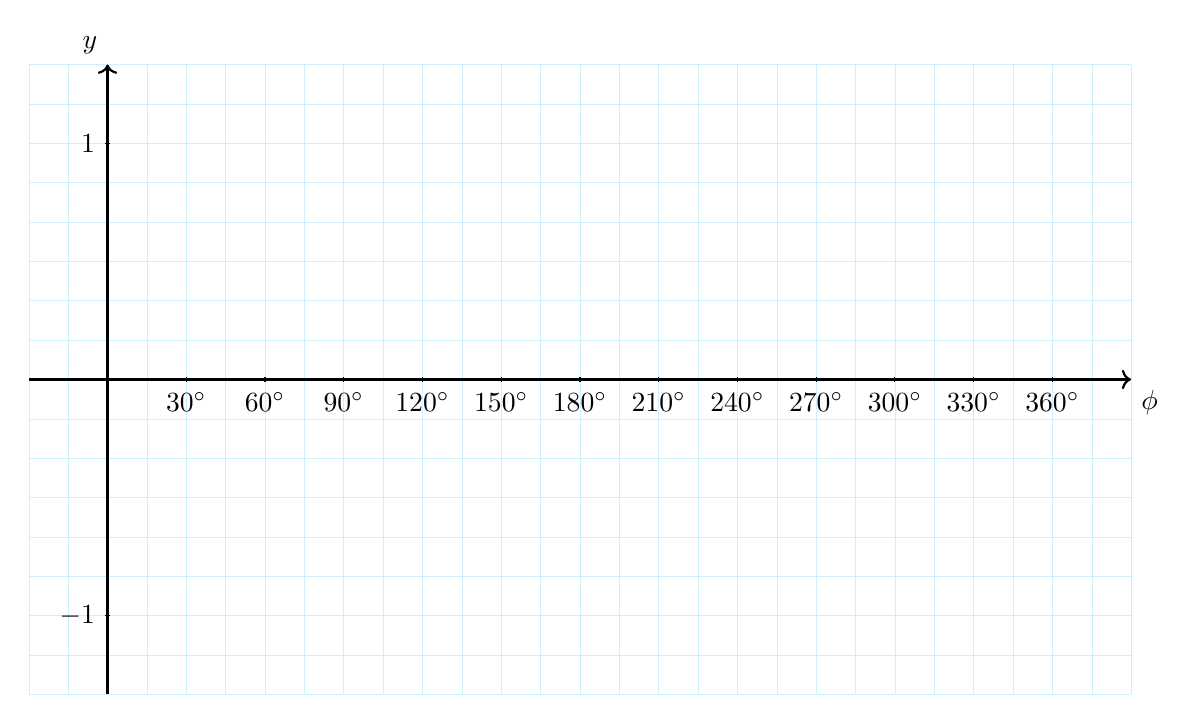
\begin{tikzpicture}\draw[step = 0.5 cm, cyan!20 , very thin] (-1, -4) grid ( 13, 4);
\draw[thick, ->] (-1,0) -- (13,0) node[anchor = north west] {$\phi$};
\draw[thick, ->] (0,-4) -- (0,4) node[anchor = south east] {$y$};

\foreach \x [evaluate=\x as \degree using int(\x*30)] in {1,...,12}{ 
   \draw (\x cm, 1pt) -- (\x cm, -1pt) node[anchor = north] {$\degree^\circ$};
   }
\foreach \y in {-1,1}
   \draw (1pt, \y *3cm) -- (-1pt, \y *3cm) node[anchor = east] {$\y$};

\end{tikzpicture}}%% END Definition

\newcommand{\trigsysC}{
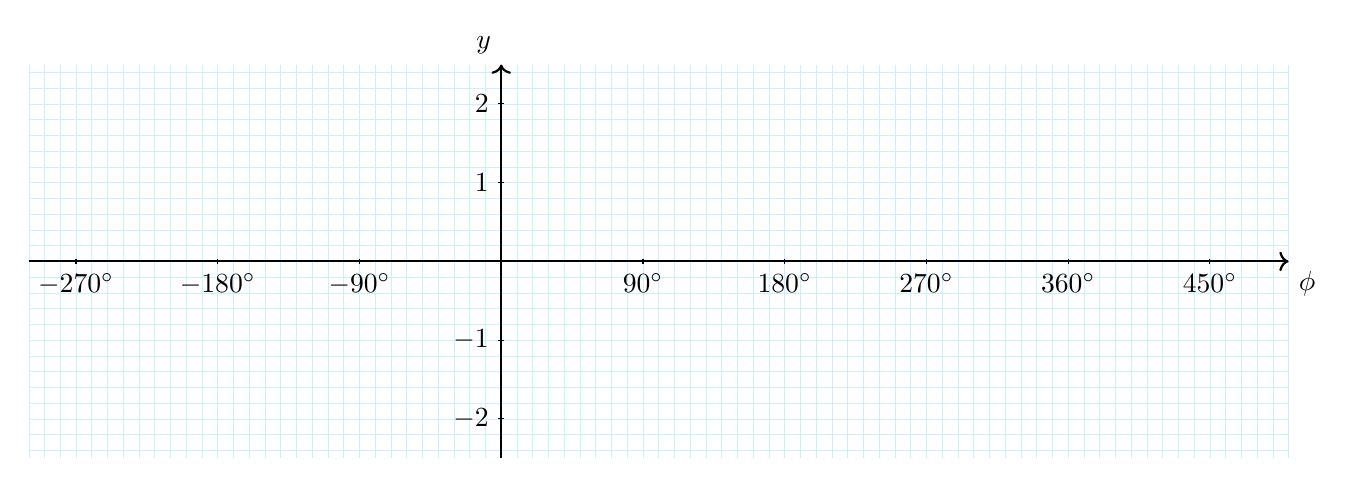
\begin{tikzpicture}
\draw[step = 0.2 cm, very thin, cyan!20] (-6, -2.5) grid ( 10, 2.5);
\draw[thick, ->] (-6,0) -- (10,0) node[anchor = north west] {$\phi$};
\draw[thick, ->] (0,-2.5) -- (0,2.5) node[anchor = south east] {$y$};

\foreach \x [evaluate=\x as \degree using int(\x*90)] in {-3,-2,-1,1,2,3,4,5}{ 
   \draw (\x *18mm, 1pt) -- (\x * 18mm, -1pt) node[anchor = north] {$\degree^\circ$};
   }
   
\foreach \y in {-2,-1,1,2}
   \draw (1pt, \y cm) -- (-1pt, \y cm) node[anchor = east] {$\y$};
\end{tikzpicture}}%% END Definition

\newcommand{\trigsysD}{
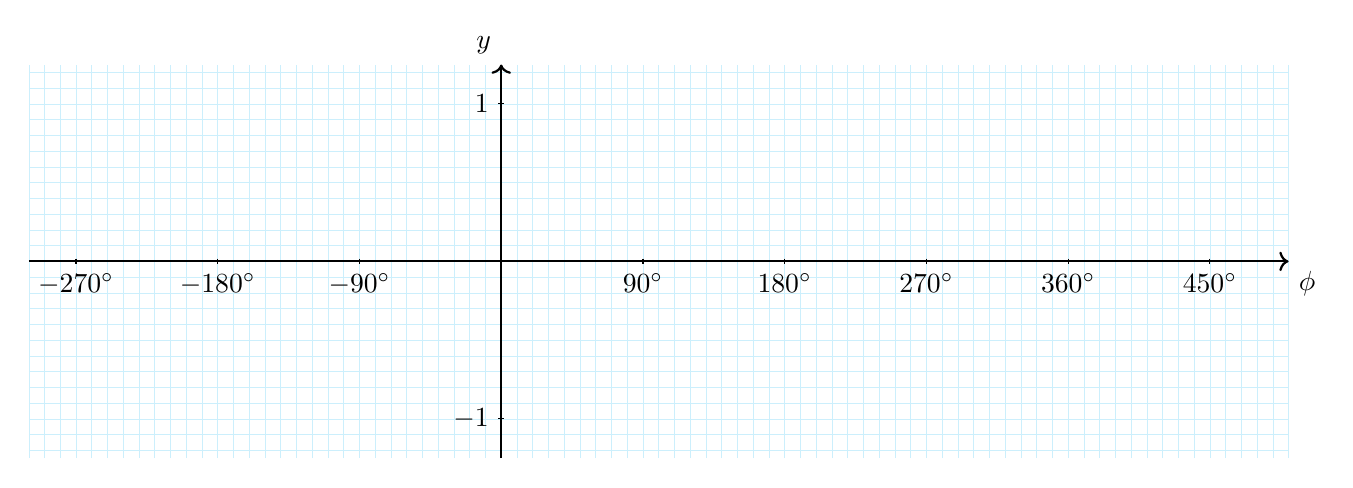
\begin{tikzpicture}
\draw[step = 0.2 cm, very thin, cyan!20] (-6, -2.5) grid ( 10, 2.5);
\draw[thick, ->] (-6,0) -- (10,0) node[anchor = north west] {$\phi$};
\draw[thick, ->] (0,-2.5) -- (0,2.5) node[anchor = south east] {$y$};

\foreach \x [evaluate=\x as \degree using int(\x*90)] in {-3,-2,-1,1,2,3,4,5}{ 
   \draw (\x *18mm, 1pt) -- (\x * 18mm, -1pt) node[anchor = north] {$\degree^\circ$};
   }
   
\foreach \y in {-1,1}
   \draw (1pt, \y *2cm) -- (-1pt, \y *2cm) node[anchor = east] {$\y$};
\end{tikzpicture}}%% END Definition


\newcommand{\trigsysDsin}{
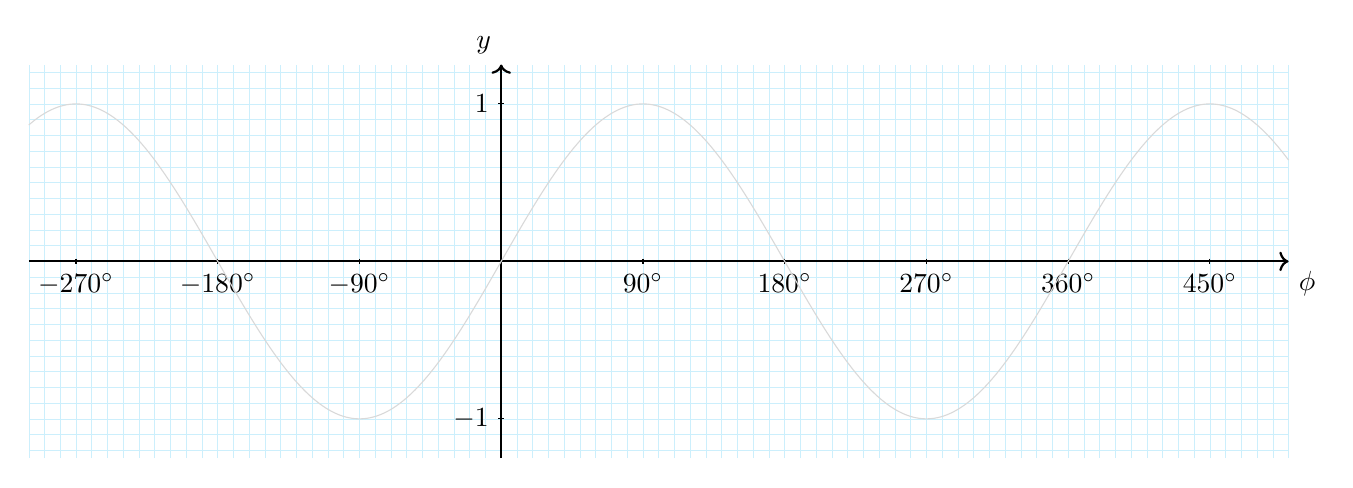
\begin{tikzpicture}
\draw[step = 0.2 cm, very thin, cyan!20] (-6, -2.5) grid ( 10, 2.5);
\draw[thick, ->] (-6,0) -- (10,0) node[anchor = north west] {$\phi$};
\draw[thick, ->] (0,-2.5) -- (0,2.5) node[anchor = south east] {$y$};

\foreach \x [evaluate=\x as \degree using int(\x*90)] in {-3,-2,-1,1,2,3,4,5}{ 
   \draw (\x *18mm, 1pt) -- (\x * 18mm, -1pt) node[anchor = north] {$\degree^\circ$};
   }
   
\foreach \y in {-1,1}
   \draw (1pt, \y *2cm) -- (-1pt, \y *2cm) node[anchor = east] {$\y$};

\draw[domain=-6:10,smooth,samples=200,variable=\x,gray!30] plot ({\x},{2*sin(\x*50)});
\end{tikzpicture}}%% END Definition

\newcommand{\trigsysDcos}{
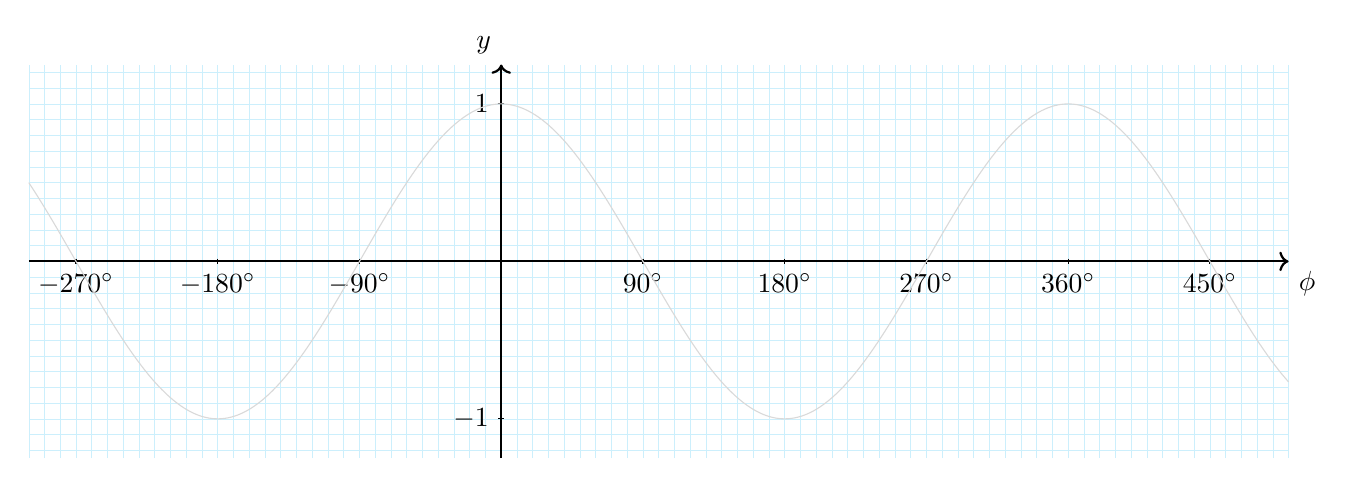
\begin{tikzpicture}
\draw[step = 0.2 cm, very thin, cyan!20] (-6, -2.5) grid ( 10, 2.5);
\draw[thick, ->] (-6,0) -- (10,0) node[anchor = north west] {$\phi$};
\draw[thick, ->] (0,-2.5) -- (0,2.5) node[anchor = south east] {$y$};

\foreach \x [evaluate=\x as \degree using int(\x*90)] in {-3,-2,-1,1,2,3,4,5}{ 
   \draw (\x *18mm, 1pt) -- (\x * 18mm, -1pt) node[anchor = north] {$\degree^\circ$};
   }
   
\foreach \y in {-1,1}
   \draw (1pt, \y *2cm) -- (-1pt, \y *2cm) node[anchor = east] {$\y$};

\draw[domain=-6:10,smooth,samples=200,variable=\x,gray!30] plot ({\x},{2*cos(\x*50)});
\end{tikzpicture}}%% END Definition




\usepackage{bbwLayoutDocSty}

%%%%%%%%%%%%%%%  H E A D E R   &   F O O T E R %%%%%%%%%%%%%%%%%%%%

%% Oben (Header) linke Seite
\fancyhf[HLE]{\makebox{
\includegraphics[width=37mm]{logos/bbwBreit.pdf}}} 
\fancyhf[HCE]{\parttitle}
%% Oben (Header) rechte Seite
\fancyhf[HRO]{\leftmark}
%% Unten (Footer)  FRE = right even, FLE= left even, FRO = right odd,
%% FCO = center odd
\fancyhf[FRE]{\doctitel{}:\ \fachthema}
\fancyhf[FLE,FRO]{\thepage{}/\pageref{LastPage}}
\fancyhf[FCO]{BBW: Abteilung 6 BMS}


\renewcommand{\author}{Philipp G. Freimann, nach Susanne Wagner und Urs Vonesch}
\renewcommand{\grafikautor}{Ph. G. Freimann}
\renewcommand{\authoremail}{philipp.freimann@bbw.ch}
\renewcommand{\erstellungsdatum}{19. Juli 2019}
\renewcommand{\docversion}{0.0.1 (\LaTeX{})}

\renewcommand{\doctitel}{Kompendium Mathematik}
\renewcommand{\untertitel}{Fachbereich Gesundheit / Soziale Arbeit}
\renewcommand{\fachthema}{Aufgaben}
\renewcommand{\rechte}{\textbf{Nutzungsrechte} Creative Commons CC-NB-CY}

%%%%%%%%%%%%%%%%%%%%%%%%%%%%%%%%%%%%%%%%%%%%%%%%%%%%%%%%%%%%%%%%%%%
%%%%%%%%%%%%%% A r i t h m e t i k   u n d   A l g e b r a  I
\begin{document}

\ptitlepage

%%\newpage
\newpage
\part{Repetitionsaufgaben}
%%
%% 2019 07 04 Ph. G. Freimann
%%


\section{Grundlagen Arithmetik und Algebra}
\input{Rep_GESO/Rechte}

\subsection{Grundlagen}
Benennen Sie die folgenden Terme mit dem richtigen Begriff
(Jeweils einer aus: \textit{Summe}, \textit{Differenz}, \textit{Produkt},
\textit{Quotient}, \textit{Potenz}):


\begin{multicols}{3}
\begin{enumerate}[label=\alph*)]
 \item $(3+x)\cdot{}2 + y$ \TRAINER{Summe}
 \item $(4a)^x$ \TRAINER{Potenz}
 \item$4a^x$ \TRAINER{Produkt}
 \item$(x-2y^4z)^2$ \TRAINER{Potenz}
 \item$2a^7 - 4bc(z-1)^3$ \TRAINER{Differenz}
 \item$(2a -b) : x + z : 4$ \TRAINER{Summe}
 \item$(a-4)(z+3)$ \TRAINER{Produkt}
 \item$(2a-b):(x+z:4)$ \TRAINER{Quotient}
\end{enumerate}
\end{multicols}

\subsubsection{Zahlmengen und zugehörige Grundoperationen}
Ordnen Sie die folgenden Zahlen der am weitesten links stehenden
Zahlmenge zu:

$$\mathbb{N} \subset \mathbb{Z} \subset \mathbb{Q} \subset \mathbb{R}$$

\begin{multicols}{2}
\begin{enumerate}[label=\alph*)]
 \item$-\sqrt{\frac{16}{2}}$ \TRAINER{$\mathbb{R}$}
 \item$|-\pi|$ \TRAINER{$\mathbb{R}$}
 \item$1.\overline{25}$ \TRAINER{$\mathbb{Q}$}
 \item$\frac{\sqrt{8}}{\sqrt{2}}$ \TRAINER{$\mathbb{N}$}
\end{enumerate}
\end{multicols}


\subsubsection{Ordnungsrelationen}
Setzen Sie zwischen die Terme (an die Stelle der drei Punkte) die
richtigen Relationszeichen ($<$, $=$, $>$):

\begin{multicols}{2}
\begin{enumerate}[label=\alph*)]
 \item$|5-2| ... |2-5|$ \TRAINER{$=$}
 \item$-\sqrt{3} ... -\sqrt{2}$ \TRAINER{$<$}
 \item$-3 ... |-3|$ \TRAINER{$<$}
 \item$\frac{1}{3} ... \frac{1}{4}$ \TRAINER{$>$}
 \item$\frac{2}{3} ... \frac{3}{4}$ \TRAINER{$<$}
 \item$2.\overline{9}$ ... 3\TRAINER{$=$}
 \item$-\frac{1}{3} ... -\frac{1}{4}$ \TRAINER{$<$}
\end{enumerate}
\end{multicols}


\subsubsection{Absolutbetrag}
Lösen Sie in der Grundmenge $\mathbb{Z}$:

\begin{multicols}{2}
\begin{enumerate}[label=\alph*)]
 \item$|x+4| = 5$ \TRAINER{$\mathbb{L}=\{1,-9\}$}
 \item$|2x-1| = 0$ \TRAINER{$\mathbb{L}=\{0.5\}$}
 \item$|-x + 7| = 10$ \TRAINER{$\mathbb{L}=\{-3, 17\}$}
 \item$|-x|=-1$ \TRAINER{$\mathbb{L}=\{\}$}
\end{enumerate}
\end{multicols}

\subsubsection{Runden}\index{Runden!Aufgaben}
Runden Sie auf 2 Dezimalen (Nachkommastellen):

\begin{multicols}{3}
\begin{enumerate}[label=\alph*)]
 \item$2.245$ \TRAINER{2.25}
 \item$2.995$ \TRAINER{3.00}
 \item$\sqrt{3}$ \TRAINER{1.73}
\end{enumerate}
\end{multicols}

Runden Sie auf vier signifikante Stellen:

\begin{multicols}{2}
\begin{enumerate}[label=\alph*)]
 \item 12.05649  \TRAINER{12.06}
 \item 0.028249 \TRAINER{0.02825}
 \item 2\,468\,900  \TRAINER{2\,469\,000}
 \item 1\,370.5   \TRAINER{1\,371}
\end{enumerate}
\end{multicols}

Runden Sie auf 2 Dezimalstellen in der wissenschaftlichen Notation:
\begin{multicols}{2}
\begin{enumerate}[label=\alph*)]
 \item 12.05649  \TRAINER{1.21 $\cdot 10^1$}
 \item 0.028249 \TRAINER{2.82 $\cdot 10^{-2}$}
 \item 2\,468\,900  \TRAINER{2.47 $\cdot 10^{6}$}
\end{enumerate}
\end{multicols}


%%%%%%%%%%%%%%%%%%%%%%%%%%%%%%%%%%%%%%%%%%%%%%%%%%
%% Summenzeichen
\subsection{Grundoperationen mit algebraischen Termen}
Schreiben Sie die Summanden hin und berechnen Sie den Wert des Ausdrucks:
\begin{enumerate}[label=\alph*)]
 \item $$\sum_{k=2}^{k=4}{(3k+2^k)}$$ \TRAINER{(6+4) + (9+8) + (12+16) = 10+17+28=55}
 \item $$\sum_{i=4}^{i=7}(3i) + 6$$   \TRAINER{((12) + (15) + (18) +(21) )+6=72}
\end{enumerate}


Schreiben Sie als Summen:

\begin{multicols}{2}
\begin{enumerate}[label=\alph*)]
\item $\left(5m-\frac{1}{2}n\right)^2$
\item $(t-9s^2)\cdot(t+9s^2)$
  \item $(3a + b^4)^2$
  \end{enumerate}
\end{multicols}

Faktorzerlegung mit Hilfe der Binomischen Formeln\index{Binomische
  Formeln!Aufgaben}

\begin{multicols}{2}
\begin{enumerate}[label=\alph*)]
\item $4x^2-y^2$
\item $36a^2 + 36ab + 9b^2$
\item $4x^4-28x^2y+49y^2$
\item $a^3-a$
\item $x^3-6x^2y+9xy^2$
  \item $z^4 -3^2$
\end{enumerate}
\end{multicols}

Faktorzerlegung durch planmäßiges Probieren

\begin{multicols}{2}
\begin{enumerate}[label=\alph*)]
\item $a^2 + 2a -15$
\item $a^3-a^2-6a$
\item $a^2 - 20a + 75$
  \item $a^2 -19a + 48$
\end{enumerate}
\end{multicols}

Faktorzerlegung durch teilweises Ausklammern und Ausklammern von
Klammern (Zerlegen Sie in möglichst viele Faktoren):

\begin{multicols}{2}
\begin{enumerate}[label=\alph*)]
\item $ab(x-2y)-b(x-2y)$
\item $x(y-2z)-(y-2z)$
\item $(a-2b)(m+n)+(a-2b)(3m+n)$
\item $3a-6ab+c-2bc$
  \item $ac-ad+bc-bd$
\end{enumerate}
\end{multicols}

Bruchterme umformen

\begin{multicols}{2}
\begin{enumerate}[label=\alph*)]
\item $\frac{st-3t^2}{s^2-st} + \frac{3s^2-3st-st+t^2}{s^2-2st+t^2}$
\item $\frac{\frac{a^2-16c^2}{8a^2}}{\frac{a-4c}{4a}}$
\item $\left(\frac{1}{a^2} - \frac{1}{b^2}\right) \cdot
    \left(\frac{a}{a+b} + \frac{b}{a-b}\right)$
\item $\left( \frac{a+4}{a} - \frac{b+4}{b}\right) : \frac{a-b}{a}$
    
\end{enumerate}
\end{multicols}


\subsection{Potenzen}

Schreiben Sie als Bruch ohne negative Exponenten:

\begin{multicols}{2}
\begin{enumerate}[label=\alph*)]
\item $2x^{-3}$
  \item $ab^{-5}$
\end{enumerate}
\end{multicols}

Schreiben Sie folgende Bruchzahlen als Dreierpotenzen:

\begin{multicols}{2}
\begin{enumerate}[label=\alph*)]
  \item $\frac{1}{9}$
  \item $\frac{1}{27}$
    \item $\frac{1}{81}$
\end{enumerate}
\end{multicols}

Lösen Sie die Exponentialgleichungen durch Erzeugen gleicher Basis:

\begin{multicols}{3}
\begin{enumerate}[label=\alph*)]
\item $2^x=\frac{1}{8}$
\item $2^{2x}=\frac{1}{8}$
\item $4^x=\frac{1}{32}$
\item $3^x=\frac{1}{81}$
  \item $9^x=\frac{1}{3}$
  \item $27^{2x}=\frac{1}{9}$
  \item $\left(3^x\right)^6 = \frac{1}{81}$
    \item $50\cdot 5^{n-1} + 3\cdot 5^{n+1} = 5^x$
    \item $\frac{25^k}{125^3} = 5^x$
      \item $2^x=\frac{8^4}{4^8}$
\end{enumerate}
\end{multicols}


Wenden Sie die Potenzgesetze an und schreiben Sie so einfach wie
möglich:
\begin{multicols}{3}
\begin{enumerate}[label=\alph*)]
\item $a\cdot a^{2x+3} : a^{1-x}$
\item $\left(\frac{x}{y}\right)^7 : \left(\frac{-x}{y}\right)^3$
\item $(-b)^6 \cdot (-b^8)$
\item $(-x^3)^4$
\item $\left( -(a^{-1})^{-2} \right)^6$
\item $(-a)^4 : (-a^{10})$
  \item $4^k \cdot \left( \frac{1}{2} \right)^k \cdot \left(
    \frac{1}{3} \right)^{-k}$
\end{enumerate}
\end{multicols}


Vereinfachen Sie:
$$\left(\frac{3x^{-2}y^2}{4x^{-4}y^3}\right)^{-2} : \left(\frac{2x^{-1}}{3xy^{-2}}\right)^3$$


Vereinfachen Sie folgende Terme. Resultat in Wurzelschreibweise:

\begin{multicols}{2}
\begin{enumerate}[label=\alph*)]
\item $\left(\frac{1}{a}\right)^{-\frac{1}{4}}$
\item $\sqrt{x}\cdot \sqrt[3]{x^4} \cdot \sqrt[6]{x^3}$
  \item $3a\cdot \sqrt[3]{9a^2}$
\item $\sqrt[4]{b\cdot \sqrt[3]{b^2\cdot \sqrt{b}}}$
\end{enumerate}
\end{multicols}

%%%%%%%%%%%%%%%%%%%%%%%%%%%%%%%%%%%%%%%%%%%%%%%%%%%%%%%%% 
\subsection{Zehnerlogarithmen}

Berechnen Sie die Exponenten. Resultate exakt, wenn nötig mit Hilfe von
Zehnerlogarithmen:

\begin{multicols}{2}
\begin{enumerate}[label=\alph*)]
\item $a^x=b$
\item $4^x=12$
  \item $4\cdot 3^{x+1}=6$
\end{enumerate}
\end{multicols}x

%%
%% 2019 07 04 Ph. G. Freimann
%%

\input{geso/Rep_GESO/Rechte}

\section{Gleichungen und Gleichungssysteme}
\subsection{Lineare Gleichungen}

\subsubsection{Erfüllbare und unerfüllbare lineare Gleichungen}

Bestimmen Sie die Lösungsmenge bezüglich der Grundmenge
$G=\mathbb{R}$:

\begin{enumerate}[label=\alph*)]
\item $4x=7+3x$
\item $3x=x$
\item $(x+2)^2 + (x+3)^2 - (x+5)^2 = (x-2)^2 - 12$
\item $6x + 5 = \frac{1}{3} (18x + 15)$
\item $8x -2 = 4x + 1 - (-4x - 3.5)$
\item $\frac{3x-1}{4} + \frac{2x+1}{5} - 1 = \frac{3x-1}{5} +6 - \frac{x+2}{3}$
\end{enumerate}

\subsubsection{Lineare Bruchgleichungen (Definitions- und
  Lösungsmenge)}

Nennen Sie die Definitionsmenge, lösen Sie anschließend die Gleichung
und bestimmen Sie die Lösungsmenge; $G=\mathbb{R}$. Exakte Werte
angeben:

\begin{multicols}{2}
\begin{enumerate}[label=\alph*)]
\item $\frac{4a+6}{2a-10} + \frac{6a-43}{5-a} = -10$
\item $\frac{22.5}{a-3} + \frac{9}{-a^2 + 6a - 9} = 0$
\item $\frac{1}{x(x-4)} + \frac{1}{x(x+4)} = \frac{2}{x^2-16}$
\item $\frac{3.6x+8.5}{x^2-x-12} + \frac{5.2}{x-4} = \frac{1.9}{-x-3}$
\item $\frac{21}{-x+7} = 3 + \frac{1.5x}{\left(\frac{7-x}{2}\right)}$    
\end{enumerate}
\end{multicols}

\subsubsection{Lineare Gleichungen mit Parametern}

Bestimmen Sie die Lösungen. Schreiben Sie die Ergebnisse so einfach
wie möglich. Die Lösungsvariable ist jeweils $x$:

\begin{enumerate}[label=\alph*)]
\item $(t+x-s)(t-x-s) = (t-x)(s+x) - st$
\item $\frac{k-bx}{v} + x = \frac{vx-b}{v}$
\item $(k-4)x = 4k - k^2$
\item $\frac{1}{x} + \frac{1}{a} = \frac{1}{b}$
  \item $\frac{x- \frac{n^2}{4}}{\frac{1}{2} - \frac{n}{4}} = x+n$

\end{enumerate}

\subsubsection{Textaufgaben, die auf lineare Gleichungen führen}

\begin{enumerate}
\item
  Zerlegen Sie die Zahl 188 so in zwei Summanden, dass der 3. Teil des
  ersten Summanden um 12 kleiner ist als der 5. Teil des zweiten
  Summanden. Wie heißen die beiden Summanden?

\item Urs addiert zu einer gedachte Zahl $x$ die Zahl 5, setzt recht
  an die Summe die Ziffer 7, dividiert die entstandene Zahl durch 11,
  multipliziert den Quotienten mit 4 und erhält das 14-fache der
  ursprünglichen Zahl. Um welche Zahl $x$ handelt es sich?

\item Jemand muss zwei Kredite von zusammen CHF 180\,000.- zu 4.5\%
  und 5.5\% verzinsen. Wären die Zinssätze vertauscht, so ergäbe sich
  ein um CHF 225.- niedriger Jahreszins. Wie hoch sind die Kredite?

\item Jemand macht per 1. Juni eine Einlage von CHF 75\,000.- bei
  einem Zinsfuß von 3.5\%. Einige Monate später erhöht sich der
  Zinsfuß um 1.5\%, so dass am Jahresende auch ein um CHF 281.25
  höherer Zins als ursprünglich erwartet resultiert. Wann fand die
  Erhöhung statt?

\item Eine Buchhandlung verkaufte von den vorhandenen Exemplaren eines
  neu erschienen Krimis am ersten Tag ein Achtel und 10 Stück, am
  zweiten Tag vom Restbestand die Hälfte und 15 Stück. Danach blieben
  noch 50 Krimis übrig. Wie viele Exemplare waren ursprünglich
  vorhanden?

\item Ein Kaufmann mischt 6\,kg einer Warensorte mit 14\,kg einer
  zweiten Sorte. Der Preis je kg der ersten Sorte ist um CHF 2.50
  höher als derjenige der zweiten Sorte. Er erhält eine Mischung, die
  CHF 8.- pro kg kostet. Wie teuer ist jede der beiden Sorten pro kg?

\item Aus 60\%-igem und 65\%-igem Alkohol sollen 150 Liter 63\%-ige
  Mischung hergestellt werden. Wie viele Liter von jeder Sorte muss
  man verwenden?

\item Auf dem Flohmarkt wird um ein Ölbild gefeilscht. Der Händler
  verlangt CHF 590.-, während der Käufer nur CHF 410.- bezahlen
  will. Die beiden einigen sich so, dass der Händler den Preis um
  gleich viele Prozente senkt, wie der Käufer sein Angebot
  erhöht. Welches ist der Verkaufspreis und um wie viele Prozente sind
  beide von ihren Forderungen abgewichen?

\item Wenn zwei Zuleitungen gleichzeitig geöffnet sind, füllen sie ein
  Bassin in 9 Minuten und 36 Sekunden. Um das Bassin alleine zu
  füllen, braucht die erste Zuleitung 12 Minuten. Wie lange benötigt
  die zweite Zuleitung, wenn sie das Bassin alleine füllen soll?

\item Eine Weinhändlerin kauft 300 Liter Rotwein und 600 Liter
  Weißwein. Der Preis pro Liter Weißwein ist um CHF 1.50 höher als der
  Literpreis Rotwein. Weil der Weinbauer und die Händlerin alte
  Freunde aus der BM-Schulzeit sind, erhält die Weinhändlerin pro
  Liter Rotwein 10\% und pro Liter Weißwein 12\% Rabatt.
  Der Weinbauer vertauscht jedoch die beiden Rabatte und schickt der
  Händlerin somit eine Rechnung, die um CHF 60.- zu hoch ist.
  Berechnen Sie die Literpreise für Rot- bzw. Weißwein vor Abzug der
  Rabattes.
\end{enumerate}


\subsection{Gleichungssysteme mit zwei Unbekannten}

  Bringen Sie die Gleichungen auf die Grundform und lösen diese
  anschließend mit dem Taschenrechnermodus.

  Bestimmen Sie die Lösungsmenge bezüglich der Grundmenge $G = \{(x,
  y) \in \mathbb{R}\times\mathbb{R}\}$;

\begin{multicols}{2}
  \begin{enumerate}
  \item
    
    \gleichungZZ{-\frac{x}{2}}{2y-1+x}{\frac{x}{2}+3}{1-x}

  \item
    \gleichungZZ{\frac{a+b}{6}}{\frac{a}{2}-5}{a+8}{\frac{b+a}{6}}

  \item
  \gleichungZZ{5x-8y}{1}{20x}{7+32y}

\item
  $$2x+7y = -5+8y = 24x +7$$
\item
  \gleichungZZ{3x}{2+5y}{6}{\frac{24}{3x} + \frac{10y}{x}}

\item
  \gleichungZZ{\frac{4x-1}{5}-x}{y-\frac{3y-4}{2}}{\frac{x+y-3}{2x-y+7}}{\frac{3}{4}}
  
  \end{enumerate}
\end{multicols}


  \subsection{Substitution (zwei Gleichungen, zwei Unbekannte)}

\begin{multicols}{2}
  \begin{enumerate}
  \item
    \gleichungZZ{\frac{b}{a+b}}{1-\frac{3}{a-b}}{\frac{3b}{a+b}}{1-\frac{2}{a-b}}

  \item
    \gleichungZZ{\frac{2y}{4x-1}+9}{\frac{5}{x+2y}}{\frac{10}{x+2y}-12}{\frac{y}{4x-1}}
  \end{enumerate}
\end{multicols}

  \subsection{Textaufgaben}

  \begin{enumerate}
  \item
    Farben der Sorte A und der Sorte B mit Kilopreisen von CHF 12.-
    bzw. CHF 10.- werden gemischt. Ein Kilogramm Mischung kommt nun
    auf CHF 10.90 zu stehen. Nähme man bei gleicher Gesamtmenge der
    Mischen von der Sorte A 3 kg weniger, so würde das Kilogramm nur
    noch CHF 10.40 kosten. Wie viele kg nahm man anfänglich von jeder
    Sorte?

    \item Frau Groß hat ein Kapital in zwei Posten angelegt, einen zu
      4\% und einen zu 5\%. Nach ihrer Rechnung beträgt die Summe der
      Jahreszinsen CHF 2\,560. Das sind aber CHF 80.- zu viel; sie hat
      nämlich die Zinssätze verwechselt. Welche Posten hat sie zu
      welchem Zinssatz angelegt?

      \item Dividiert man eine zweiziffrige Zahl durch ihre Quersumme,
        so erhält man 4 Rest 9. Vertauscht man die Ziffern der
        ursprünglichen Zahl und dividiert diese durch die um 13
        vermehrte Quersumme, so erhält man 3.


        \item Eine Händlerin kaufte 800 Stück von Sorte I und 400
          Stück von Sorte II für insgesamt CHF 4\,200. Sorte I
          verkaufte sie mit einem Zuschlag von 15\% und Sorte II mit
          einem Zuschlag von 50\%. Der Verkaufspreis betrug insgesamt
          CHF 5\,180. Für wie viel Geld hatte sie ein Stück jeder
          Sorte eingekauft?
          
    \end{enumerate}


  \subsection{graphisches Lösen von linearen Gleichungssystemen}

  \begin{enumerate}
  \item Lösen Sie das Gleichungssystem grafisch für
    $-20 \leq x \leq 80$ und $-50 \leq y \leq 100$.

    \gleichungZZ{10y}{7.5x}{18.75x+25y}{1500}

    \item Lösen Sie das Gleichungssystem grafisch für
      $-10 \leq x \leq 10$ und $-10 \leq y \leq 10$.

      \gleichungZZ{3x+y-9.5}{4y-\frac{28}{7}}{-\frac{4}{5}y + x}{-5+0.2x}

          \item Lösen Sie das Gleichungssystem grafisch für
      $-50 \leq x \leq 50$ und $-50 \leq y \leq 50$.

            \gleichungZZ{40}{-2y-x}{3.5x -5y +82}{4\left(x-y+\frac{51}{2}\right)}

  \end{enumerate}


  \subsection{Quadratische Gleichungen}

  Lösen Sie die Gleichungen ohne Solve-Funktion des Taschenrechners,
  indem Sie sie auf die Grundform bringe. Die Grundform kann
  anschließend mit dem entsprechenden Taschenrechnermodus gelöst
  werden.

  \subsubsection{Reinquadratische Gleichungen}
  Bestimmen sie $x$:
  \begin{multicols}{2}
  \begin{enumerate}
  \item $x^2 = 0.04$
  \item $x^2+4=0$
  \item $(7+x)(7-x)=(3x+2)^2-(2x+3)^2$
    \item $\frac{x-3}{x+3} + \frac{x+3}{x-3} = \frac{26}{x^2-9}$
  \end{enumerate}
  \end{multicols}

  \subsubsection{Gemischtquadratische Gleichungen: Lösungsformel}
  Grundform:

  \begin{tabular}{|c|c|}%%
    \hline%%
Grundform: $ax^2 + bx +c = 0$ & Lösungsformel: $x_{1,2} = \frac{-b \pm \sqrt{b^2 - 4ac}}{2a}$\\%%
    \hline%%
    \end{tabular}%%

  Bestimmen Sie $x$:
  \begin{multicols}{3}
  \begin{enumerate}
  \item $0 = 12x^2 - 8x - \frac{4}{3}$
  \item $3x^2 + 5x = -1$
  \item $-5x^2 = 20 + 7.5x$
  \item $\frac{1}{8}x^2 + 2.5x + 8 = 0$
  \item $\frac{x-4}{x-5} = \frac{30-x^2}{x^2-5x}$
    \item $\frac{x}{3} - \frac{x^2-19}{3x+6} = 3 + \frac{4x-7}{6-3x}$
    \end{enumerate}
    \end{multicols}

  \subsubsection{Quadratische Gleichungen: Substitution}
  Gleichungen höheren Grades, die durch Substitution auf eine
  quadratische Gleichung führen:

  \begin{enumerate}
  \item Lösen Sie die Gleichung nach $x$ auf. Resultate exakt:
    $$\left(x-\frac{3}{x}\right)^2 - 20 = x - \frac{3}{x}$$

  \item Lösen Sie die Gleichung nach $x$ auf und runden Sie das
    Resultat auf drei Dezimalstellen:
    $$(x+7)^6 = 8\cdot (x+7)^3 - 15$$

  \item $$(x+7)^8 = 14(x+7)^4 + 32$$
  \end{enumerate}


    \subsection{Textaufgaben, die auf quadratische Gleichungen führen}
Die Gleichungen sind auf Grundform zu bringen und können anschließend
mit dem entsprechenden Taschenrechnermodus gelöst werden.

\begin{enumerate}
  \item Ein Speicher wird durch eine Zuleitung in einer bestimmten
    Zeit gefüllt. Das Entleeren durch eine andere Leitung dauert eine
    Minute länger. Aus Unachtsamkeit bleibt während des Füllens die
    andere Leitung geöffnet, deshalb ist der Speicher erst nach 756
    Minuten voll. Wie lange dauert die Leerung des Speichers bei
    geschlossener Zuleitung?

    \item Das Produkt der beiden kleinsten von sechs aufeinander
      folgenden natürlichen Zahlen ist dreimal so groß wie die Summe
      der vier übrigen Zahlen. Wie heißt die kleinste Zahl?

      \item Eine Praxiseinrichtung mit einem Anschaffungswert von CHF
        24\,000;.- wurde zweimal mit dem gleichen Prozentsatz
        abgeschrieben und hat zur Zeit einen Wert von CHF 16\,335.-.
        Wie viele Prozente beträgt der Abschreibungssatz?

      \item Dividiert man die Summe zweier positiver Zahlen durch ihre
        Differenz, so erhält man 12.5\% der größeren Zahl.
        Berechnen Sie die größere Zahl, wenn die kleinere 42 ist.

        \item Die Zehnerziffer einer zweiziffrigen Zahl ist um 6
          kleiner als die Einerziffer. Die vierfache Summe der
          Quadrate der Ziffern ist gleich der fünfunzwanzigfachen
          Quersumme. Wie heißt die Zahl?
\end{enumerate}


\subsection{Elementare Potenzgleichungen mit ganzzahligen und
  rationalen Exponenten}
Lösen Sie die Gleichung ohne Solve-Funktion des Taschenrechners nach
$x$ auf und schreiben Sie die Resultate als exakte Werte ($G =
\mathbb{R}$):

\begin{multicols}{3}
\begin{enumerate}
\item $\frac{2}{3}x^3 = 12$
\item $x^5 = \frac{1}{32}$
\item $\left(\frac{1}{x}\right)^6 = 13$
\item $\left(\frac{x-5}{3}\right)^3=64$
\item $(x+5)^{\frac{1}{2} = 4}$
\item $\left(x-6\right)^{\frac{1}{3}} = 2$
\end{enumerate}
\end{multicols}


  \subsection{Elementare Exponentialgleichungen}
Lösen Sie die Gleichung ohne Solve-Funktion des Taschenrechners nach
$x$ auf und schreiben Sie die Resultate als exakte Werte ($G =
\mathbb{R}$).
Tipp: Erzeugen gleicher Basis

\begin{multicols}{3}
\begin{enumerate}
\item $2^x=16$
\item $\left(\frac{1}{4}\right)^x = 64$
\item $2^x\cdot 8^{x-1} = 32$
  \item $\left(\frac{1}{3}\right)^x\cdot \left(\frac{3}{27}\right)^x = 3$
  \item $e^{2x}=1$
  \item $\frac{6^{x-2}}{36^{x+1}} = 216$
  \item $\left(3^x\right)^6=\frac{1}{81}$
    \item $2^x + 2^{x+3} = \frac{9}{4}$
  \end{enumerate}
\end{multicols}

\input{Rep_GESO/Datenanalyse}

%%%%%%%%%%%%%%%%%%%%%%%%%%%%%%%%%%%%%%%%%%%%%%%%%%%%%%%%%%%%%%%%%%%
%%\newpage\mbox{}
%%\blankOddPage{}%
%\include{texlife-bibtex-extra}
 \bibliography{bibAll}{}\label{literatur}

 \printindex
%%%%%%%%%%%%%%%%%%%%%%%%%%%%%%%%%%%%%%%%%%%%%%%%%%%%%%%%%%%%%%%%%%%

\end{document}
